\documentclass{article}
\usepackage{graphicx} % Required for inserting images
\usepackage[margin=2.54cm]{geometry}
\usepackage{amsmath} % For mathematical symbols and environments
\usepackage{biblatex} %Imports biblatex package
\usepackage{mathtools}
\usepackage{physics}
\usepackage[final]{listings}

\usepackage{xcolor}

\definecolor{backcolour}{RGB}{245,245,245}
\definecolor{commentcolour}{rgb}{0,0.6,0}
\definecolor{stringcolour}{rgb}{0.58,0,0.82}
\definecolor{white}{rgb}{1,1,1}



\lstloadlanguages{Python}
\lstdefinestyle{input}{
    keywordstyle=\color{blue},
    backgroundcolor=\color{backcolour},
    stringstyle = \color{stringcolour},
    commentstyle=\color{commentcolour},
    basicstyle=\ttfamily\small,
    breakatwhitespace=false,         
    breaklines=true,                 
    captionpos=b,                    
    keepspaces=true,                 
    numbers=none,                    
    numbersep=5pt,                  
    showspaces=false,                
    showstringspaces=false,
    showtabs=false,                  
    tabsize=2
  }
  \lstdefinestyle{output}{
    backgroundcolor=\color{white},
    keywordstyle = \color{black},
    basicstyle=\ttfamily\small,
    breakatwhitespace=false,         
    breaklines=true,                 
    captionpos=b,                    
    keepspaces=true,                 
    numbers=none,                    
    numbersep=5pt,                  
    showspaces=false,                
    showstringspaces=false,
    showtabs=false,                  
    tabsize=2
}
\lstset{
    style = input,
    language = Python
}

\addbibresource{dl-ref.bib} %Import the bibliography file

\title{Deep Learning}
\author{Mairi Hallman}
\date{May 2024}

\begin{document}

\maketitle

\newpage

\tableofcontents
\newpage

\section{Introduction}

\section{A Brief Overview of Tensors}

You are likely familiar with scalars, vectors, and matrices. These can be thought of as analagous data structures in zero, one, and two-dimensions, respectively. When generalizing to \(N\) dimensions, we refer to these collectively as tensors. A scalar is a zero-order tensor, a vector is a first-order tensor, and a matrix is a second-order tensor. A third-order tensor can be visualized as a stack of matrices. A fourth-order tensor would then be a vector of third order tensors. A fifth-order tensor is a matrix of third-order tensors... and so on.

% notation

% fiber and slices

\subsection{Tensor Products}

Tensor additon and subtraction are self-explanatory if matrix addition and subtraction are understood. The same cannot be said for tensor products. Below is an overview of tensor products necessary for the decompositions that will be presented in the next section.

\subsubsection{Outer Product \(\circ\)}

A tensor \(T^{(N)}\) can be expressed as a product of \(N\) vectors. This is called the outer product (denoted \(\circ\)).

\begin{equation}
    T^{(N)} = u_1 \circ u_2 \circ \dots \circ u_N
\end{equation}

% make less hand-wavey

\subsubsection{Kronecker Product \(\otimes\)}

The Konecker product of two matrices \(A\) and B, their Kronecker product is a matrix of the products of each element in \(A\) and the entire matrix \(B\).

\begin{equation}
    A \otimes B = \begin{bmatrix}
    a_{11}B & a_{12}B & \dots & a_{1n}B \\
    a_{21}B & a_{22}B & \dots & a_{2n}B \\
    \vdots & \vdots & \ddots & \vdots \\
    a_{m1}B & a{m2}B & \dots & a_{mn}B \end{bmatrix}
    \label{Kronecker} 
\end{equation}

\subsubsection{Khatri-Rao Product \(\odot\)}

The Khatri-Rao product of two matrices \(A\) and \(B\), each with the same number of columns, is a matrix composed of the Kronecker products of the columns in matrix \(A\) and the columns in matrix \(B\) with the same indices.

\begin{equation}
    A^{:\times n} \odot B^{:\times n} = \begin{bmatrix}
    a_{:,1} \otimes b_{:,1} & a_{:,2} \otimes b_{:,2} & \dots & a_{:,n} \otimes b_{:,n} \end{bmatrix}
    \label{Khatri-Rao}
\end{equation}

\subsubsection{Hadamard Product \(*\)}

The Hadamard product of two matrices \(A\) and \(B\) of the same dimensions is a matrix formed of the products of the elements in \(A\) and \(B\) with the same indices.

\begin{equation}
    A^{m \times n} * B^{m \times n} = \begin{bmatrix}
    a_{11}b_{11} & a_{12}b_{12} & \dots & a_{1n}b_{1n} \\
    a_{21}b_{21} & a_{22}b_{22} & \dots & a_{2n}b_{2n} \\
    \vdots & \vdots & \ddots & \vdots \\
    a_{m1}b_{m1} & a_{m2}b_{m2} & \dots & a_{mn}b_{mn} \end{bmatrix} 
    \label{Hadamard}
\end{equation}

\subsection{Tensor Decompositions}

% add intro

\subsubsection{CP Decomposition}

The canonical polyadic, or CP Decomposition, decomposes a tensor into vectors.

\begin{equation}
    T = \sum_{r-1}^R u_r^{(1)} \circ  u_r^{(2)} \circ \dots  u_r^{(R)}\
    \label{CP}
\end{equation} % review notation

% add info re computation

\subsubsection{Tucker Decomposition}

The Tucker decomposition decomposes a tensor into a core tensor and factored matrices. % add more explanantion

\begin{equation}
    T = C\prod_{n=1}^N A^n
    \label{Tucker}
\end{equation} % review notation

where \(C\) is the core tensor.

% add info re computation

\subsubsection{Tensor Train}

The tensor train decomposition decomposes a tensor into a product of third-order tensors. It is used when a tensor is too large for the CP decomposition to be practical. 

% add representative equation, info on computation

\section{Architecture Design}

% intro blah blah "In section 21.4.3, we introduced neural networks..."

\subsection{Why Deep Networks} % see Probabilistic ML 13.2.5

Deep networks can often approximate complex functions with far fewer nodes than a shallow network. This is because the number of linear regions in the network grows exponentially with the number of layers \cite{montufar2014}.

To illustrate, consider a network with 5 layers, each with 10 nodes for a total of 50 nodes. For the sake of this example, we will assume that each layer has one input. The number of linear regions that can be learned by this network is \(10^5\). For a single-layer network to learn \(10^5\) linear regions, it would require \(10^5\) nodes. 

\subsection{Hidden Units and Activation Functions} % see Deep Learning 6.3; Probabilistic ML 13.2.3

Different types of hidden units serve different purposes within deep networks. Most types of hidden units perform an affine  transformation on the layer's input, and then apply an activation function \(g(z)\) to the transformed inputs \cite{Goodfellow-et-al-2016}. If all activation functions within a deep network are linear, then the network reduces to a linear model \cite{pml1Book}. While linear activation functions can be useful for reducing the number of parameters in a model , the discussion surrounding hidden units and their activation functions within a deep network typically concerns non-linear units \cite{Goodfellow-et-al-2016}. 

\subsubsection{ReLU}

In modern deep networks, the default most commonly used activation function for hidden layer is the rectified linear unit, or ReLU activation function.

\begin{equation}
    a(z) = max(0, z)
    \label{ReLU-activation}
\end{equation}

This is analagous to a linear activation function with negative inputs "turned off" \cite{pml1Book}. 

Notice that this function isn't differentiable at zero. In theory, this should make ReLU useless for gradient-based learning. In practice, most deep networks don't achieve a loss of zero, so this typically isn't a problem.

Variations of ReLU typically modify the slope for negative inputs \cite{Goodfellow-et-al-2016}. For a given input \(z_i\), this can be generalized as

\begin{equation}
    a(z,\alpha)_i = max(0, z_i) + \alpha_i min(0,z_i)
    \label{generalization-ReLU}
\end{equation}

Several ReLU variations of this form are listed below.

\paragraph{Absolute value rectification}\(\alpha = -1\); commonly used for image processing \cite{Goodfellow-et-al-2016}.

\paragraph{Leaky ReLU}\(\alpha\) is a small positive value. Leaky ReLU is used in place of standard ReLU to prevent the "dying ReLUs" problem. Units using ReLU as an activation "die" when all of the inputs are non-positive. All negative inputs results in all zero outputs, and the weights can't be updated \cite{hands-on-ml}.

\paragraph{Parametric Leaky ReLU}Leaky ReLU where \(alpha\) is learned by the model \cite{hands-on-ml}.

\subsubsection{The Sigmoid and Hyperbolic Tangent Functions}

In the early days of deep learning, two commonly used activation functions for hidden units were the sigmoid function

\begin{equation}
    a(z) = \sigma (z) = \frac{1}{1 + e^{-z}}
    \label{sigmoid-activation}
\end{equation}

and the hyperbolic tangent function

\begin{equation}
    a(z) = tanh(z)
    \label{tanh-activation}
\end{equation}

These activation functions are no longer recommended for hidden units because they saturate. The sigmoid function saturates at zero and one, and the hyperbolic tangent function saturates at  negative one and one. Saturation is problematic because it leads to the gradient of a layer's output with respect to its input. Recall what we know about backpropagation from section 21.4.3. If the gradient is close to zero, the weights will update very slowly, if at all. Without a gradient, the model can't converge to a solution. This phenomenon is known as the vanishing gradient problem.



\section{Training Deep Neural Networks} % doing hand-written rough notes first

\subsection{Hyperparameter Tuning}


\subsection{Regularization} % see Deep Learning all 7.1, 7.6, maybe 7.7, 7.8, probably 7.9, 7.12; Probabilistic ML 13.5

\subsubsection{Weight Decay} % L2: DL 7.1.1, PML 13.5.2 and L1: DL 7.1.2

Recall ridge and LASSO regression from section 20.2.4. When generalized beyond linear models, these regularization techniques are known respectively as \(\it{L}^2\) and \(\it{L}^1\) regularization. In the context of neural networks, these methods are both commonly referred to as weight decay. Weight decay applies a regularization term to the objective function \(J(\vb*{w})\). The regularized objective function \(\tilde{J}(\vb*{w})\) is 

\begin{equation}
    \tilde{J}(\vb*{w}) = J(\vb*{w}) +\frac{\lambda}{2}\norm{w}^2_2
    \label{L2-reg}
\end{equation} for \(\it{L}^2\) weight decay, and 

\begin{equation}
    \tilde{J}(\vb*{w}) = J(\vb*{w}) +\lambda\norm{w}_1
    \label{L1-reg}
\end{equation} for \(\it{L}^1\) weight decay, where \(\lambda\) is a hyperparameter.

\subsubsection{Early Stop} % DL 7.8

\subsubsection{Dropout} % DL 7.12, PML 13.5.4

% \subsubsection{Unsupervised Pretraining} idk where to put this

\subsubsection{Semi-Supervised Learning} % DL 7.6

\subsection{Optimization} % See Deep Learning all 8.3, 8.4, all 8.5, 8.7.1, 8.7.4

\subsubsection{Batch Normalization}

\subsubsection{Layer Normalization}


\section{Convolutional Neural Networks}

% add intro

\subsection{What Is Convolution?}

Many young people who are active on social media use filters on their pictures before posting them. These filters apply different effects to the photo, such as blurring, making the image black and white, or adding cartoon-like effects. When you apply a filter to a photo, you are using convolution. Convolution is an operation that takes the aggregation of the element-wise product of a tensor of input data and a (typically smaller) tensor, called a kernel. This produces a feature map. In the context of image processing, the original image is the input data, the filter is the kernel, and the filtered image is the feature map. 

This is an example of discrete convolution, which is the case that we will be primarily concerned with. % In the interest of providing a complete resource, equations for discrete and continuous convolution in one dimension are provided below \cite{Goodfellow-et-al-2016}.

In one dimension, discrete convolution is denoted
\begin{equation}
    \underbrace{s(i)}_{\substack{\text{feature} \\ \text{map}}} = (x*y)(i) = \sum\limits_{\substack{m}} \underbrace{x(m)}_{\substack{\text{input} \\ \text{data}}}\underbrace{y(i-m)}_\text{kernel}
    \label{1D-discrete-convolution}\
\end{equation}


% In the continuous case, equation \ref{1D-discrete-convolution} becomes
% \begin{equation}
    % s(i) = (x*y)(i) = \int_m x(m)y(i-m)dm
    % \label{1D-continuous-convolution}\
% \end{equation}

One of the most common applications of CNNs is in digital image processing. In the case of a black and white image, the input data is a two-dimensional tensor. Discrete convolution in two dimensions can be performed as follows \cite{Goodfellow-et-al-2016}. %check this

\begin{equation}
    s(i,j) = (x*y)(i,j)\sum\limits_{\substack{m}}\sum\limits_{\substack{n}} x(i,j)y(i-m,j-n)
    \label{2D-discrete-convolution}
\end{equation}

Since convolution is commutative, equation \ref{flipped-2D-discrete-convolution} also holds. 

\begin{equation}
    s(i,j) = (y*x)(i,j)\sum\limits_{\substack{m}}\sum\limits_{\substack{n}} x(i-m,j-n)y(i,j)
    \label{flipped-2D-discrete-convolution}
\end{equation}

Two-dimensional discrete convolution is equivalent to reversing the row and column indices of the kernel, performing element-wise multiplication, and taking the sum of the products. In the context of deep learning, the term ``convolution" often refers to a similar operation called cross-correlation (equation). This is equivalent to convolution without the reversing of the matrix indices \cite{Goodfellow-et-al-2016}. 

\begin{equation}
    s(i,j) = (y*x)(i,j)\sum\limits_{\substack{m}}\sum\limits_{\substack{n}} x(i+m,j+n)y(i,j)
    \label{cross-correlation}
\end{equation}

\subsection{How Convolution is Used in Deep Neural Networks}

Since one kernel can only extract one feature, each convolutional layer in a network uses multiple kernels. CNNs can be very computationally expensive to train, so we often skip over positions in the kernels to reduce training time. The width of the kernel and the size of the output can also be controlled by zero padding the input. Without zero padding, the output of each later would continue to shrink. The number of rows/columns per convolution is referred to as the stride of the convolution operation \cite{Goodfellow-et-al-2016}. % check this


\subsection{The Convolutional Layer}

The convolutional layers used in a CNN have three steps \cite{Goodfellow-et-al-2016}.

\begin{enumerate}
    \item Several parallel convolutions yield a set of linear activations.
    \item Each linear activation function is run through a non-linear activation function, such as ReLU. This introduces non-linearity and gives the network more flexibility. % fact-check this
    \item A pooling function replaces the output at a given location with a summary statistic of nearby outputs. One common pooling function is the max pooling function, which provides the maximum output within a rectangular neighbourhood. Pooling is useful when we only care about whether a feature is present and not its specific location. It is also helpful when processing different-sized inputs.
\end{enumerate}

The output of each layer is then used as input to the next layer.
% discrete case: \((a * b)_n = \sum\limits_{\substack{i,j \\ i+j=n}} a_i \cdot b_j\)

\subsection{Image Classification Example}

In this example, we will use convolutional neural networks to perform image classification on the Rock Paper Scissors dataset. 

\lstinputlisting[firstline=14, lastline=21 ]{dl-scripts/cnn-ex1-colab.py}

The dataset is only partitioned into training and test sets, so we set aside 30\% of the training set as a validation set.

\lstinputlisting[firstline=25, lastline=30]{dl-scripts/cnn-ex1-colab.py}

Next, we normalize by dividing by 255 and resize the images to 128x128. We also shuffle the training data to ensure that the model doesn't learn its order, and batch the training, validation, and test data.

\lstinputlisting[firstline=34, lastline=44]{dl-scripts/cnn-ex1-colab.py}

We start with a simple network with one comvolutional layer with 16 filters and a 3x3 kernel.

\lstinputlisting[firstline=48,lastline=62]{dl-scripts/cnn-ex1-colab.py}

Before fitting our model, we add an early stop mechanism to prevent overfitting.

\lstinputlisting[firstline=66,lastline=75]{dl-scripts/cnn-ex1-colab.py}

\begin{lstlisting}[style=output]
Epoch 1/10
56/56 [==============================] - 10s 85ms/step - loss: 1.0240 - accuracy: 0.7137 - val_loss: 0.2209 - val_accuracy: 0.9563
Epoch 2/10
56/56 [==============================] - 5s 61ms/step - loss: 0.0743 - accuracy: 0.9881 - val_loss: 0.0240 - val_accuracy: 0.9947
Epoch 3/10
56/56 [==============================] - 4s 37ms/step - loss: 0.0131 - accuracy: 0.9989 - val_loss: 0.0148 - val_accuracy: 0.9947
Epoch 4/10
56/56 [==============================] - 4s 37ms/step - loss: 0.0045 - accuracy: 1.0000 - val_loss: 0.0062 - val_accuracy: 0.9987
Epoch 5/10
56/56 [==============================] - 5s 58ms/step - loss: 0.0020 - accuracy: 1.0000 - val_loss: 0.0042 - val_accuracy: 1.0000
Epoch 6/10
56/56 [==============================] - 4s 38ms/step - loss: 0.0013 - accuracy: 1.0000 - val_loss: 0.0039 - val_accuracy: 1.0000
Epoch 7/10
56/56 [==============================] - 4s 38ms/step - loss: 0.0010 - accuracy: 1.0000 - val_loss: 0.0041 - val_accuracy: 0.9987
Epoch 8/10
53/56 [===========================>..] - ETA: 0s - loss: 8.3814e-04 - accuracy: 1.0000Restoring model weights from the end of the best epoch: 5.
56/56 [==============================] - 5s 59ms/step - loss: 8.2481e-04 - accuracy: 1.0000 - val_loss: 0.0032 - val_accuracy: 0.9987
Epoch 8: early stopping
\end{lstlisting}

Training accuracy of 100\% and validation accuracy of over 99\%? If something seems too good to be true, it probably is. Let's evaluate on the test data.

\lstinputlisting[firstline=79,lastline=79]{dl-scripts/cnn-ex1-colab.py}

\begin{lstlisting}[style=output]
12/12 [==============================] - 1s 104ms/step - loss: 1.3345 - accuracy: 0.7151
[1.3345420360565186, 0.7150537371635437] 
\end{lstlisting}

As expected, no such luck. What happens when we add another convolutional layer?

\lstinputlisting[firstline=83,lastline=98]{dl-scripts/cnn-ex1-colab.py}

\begin{lstlisting}[style=output]
 Epoch 1/10
 56/56 [==============================] - 6s 43ms/step - loss: 1.4043 - accuracy: 0.5890 - val_loss: 0.4816 - val_accuracy: 0.9206
 Epoch 2/10
 56/56 [==============================] - 5s 54ms/step - loss: 0.2150 - accuracy: 0.9552 - val_loss: 0.0609 - val_accuracy: 0.9881
 Epoch 3/10
 56/56 [==============================] - 4s 38ms/step - loss: 0.0441 - accuracy: 0.9909 - val_loss: 0.0182 - val_accuracy: 0.9987
 Epoch 4/10
 56/56 [==============================] - 4s 39ms/step - loss: 0.0143 - accuracy: 0.9977 - val_loss: 0.0076 - val_accuracy: 0.9987
 Epoch 5/10
 56/56 [==============================] - 5s 60ms/step - loss: 0.0053 - accuracy: 0.9994 - val_loss: 0.0030 - val_accuracy: 1.0000
 Epoch 6/10
 56/56 [==============================] - 4s 41ms/step - loss: 0.0022 - accuracy: 1.0000 - val_loss: 0.0019 - val_accuracy: 1.0000
 Epoch 7/10
 56/56 [==============================] - 4s 39ms/step - loss: 0.0016 - accuracy: 1.0000 - val_loss: 0.0013 - val_accuracy: 1.0000
 Epoch 8/10
 56/56 [==============================] - 5s 60ms/step - loss: 9.5238e-04 - accuracy: 1.0000 - val_loss: 0.0011 - val_accuracy: 1.0000
 Epoch 9/10
 56/56 [==============================] - 4s 38ms/step - loss: 6.9435e-04 - accuracy: 1.0000 - val_loss: 8.4804e-04 - val_accuracy: 1.0000
 Epoch 10/10
 56/56 [==============================] - 4s 38ms/step - loss: 5.3139e-04 - accuracy: 1.0000 - val_loss: 7.7833e-04 - val_accuracy: 1.0000

\lstinputlisting[firstline=100,lastline=100]{dl-scripts/cnn-ex1-colab.py}

\begin{lstlisting}[style=output]
12/12 [==============================] - 0s 16ms/step - loss: 1.0663 - accuracy: 0.7634
[1.0662583112716675, 0.7634408473968506]
\end{lstlisting}

An improvement, but still not amazing. Would a third convolutional layer help?

\lstinputlisting[firstline=104,lastline=121]{dl-scripts/cnn-ex1-colab.py}


\begin{lstlisting}[style=output]
 Epoch 1/10
 56/56 [==============================] - 7s 44ms/step - loss: 0.6999 - accuracy: 0.7035 - val_loss: 0.1999 - val_accuracy: 0.9101
 Epoch 2/10
 56/56 [==============================] - 4s 39ms/step - loss: 0.0600 - accuracy: 0.9864 - val_loss: 0.0188 - val_accuracy: 0.9934
 Epoch 3/10
 56/56 [==============================] - 5s 53ms/step - loss: 0.0240 - accuracy: 0.9949 - val_loss: 0.0071 - val_accuracy: 1.0000
 Epoch 4/10
 56/56 [==============================] - 4s 39ms/step - loss: 0.0022 - accuracy: 1.0000 - val_loss: 0.0011 - val_accuracy: 1.0000
 Epoch 5/10
 56/56 [==============================] - 4s 41ms/step - loss: 7.2477e-04 - accuracy: 1.0000 - val_loss: 7.4349e-04 - val_accuracy: 1.0000
 Epoch 6/10
 56/56 [==============================] - 5s 63ms/step - loss: 4.0359e-04 - accuracy: 1.0000 - val_loss: 3.2628e-04 - val_accuracy: 1.0000
 Epoch 7/10
 52/56 [==========================>...] - ETA: 0s - loss: 2.2042e-04 - accuracy: 1.0000Restoring model weights from the end of the best epoch: 4.
 56/56 [==============================] - 4s 39ms/step - loss: 2.1410e-04 - accuracy: 1.0000 - val_loss: 3.2290e-04 - val_accuracy: 1.0000
 Epoch 7: early stopping
\end{lstlisting}

\lstinputlisting[firstline=123,lastline=123]{dl-scripts/cnn-ex1-colab.py}

\begin{lstlisting}[style=output]
12/12 [==============================] - 0s 10ms/step - loss: 1.1395 - accuracy: 0.7930
[1.1395031213760376, 0.7930107712745667]
\end{lstlisting}

A slight improvement. What about a fourth layer?

\lstinputlisting[firstline=127,lastline=146]{dl-scripts/cnn-ex1-colab.py}

\begin{lstlisting}[style=output]
Epoch 1/10
56/56 [==============================] - 6s 46ms/step - loss: 0.7071 - accuracy: 0.6604 - val_loss: 0.1421 - val_accuracy: 0.9563
Epoch 2/10
56/56 [==============================] - 5s 40ms/step - loss: 0.0583 - accuracy: 0.9853 - val_loss: 0.0080 - val_accuracy: 0.9987
Epoch 3/10
56/56 [==============================] - 4s 39ms/step - loss: 0.0057 - accuracy: 0.9983 - val_loss: 0.0020 - val_accuracy: 1.0000
Epoch 4/10
56/56 [==============================] - 4s 48ms/step - loss: 0.0026 - accuracy: 0.9989 - val_loss: 0.0017 - val_accuracy: 1.0000
Epoch 5/10
56/56 [==============================] - 5s 40ms/step - loss: 0.0038 - accuracy: 0.9994 - val_loss: 0.0136 - val_accuracy: 0.9921
Epoch 6/10
56/56 [==============================] - 4s 41ms/step - loss: 0.0018 - accuracy: 0.9994 - val_loss: 2.4979e-04 - val_accuracy: 1.0000
Epoch 7/10
56/56 [==============================] - 4s 43ms/step - loss: 1.2425e-04 - accuracy: 1.0000 - val_loss: 1.3199e-04 - val_accuracy: 1.0000
Epoch 8/10
56/56 [==============================] - 5s 39ms/step - loss: 9.3137e-05 - accuracy: 1.0000 - val_loss: 9.6794e-05 - val_accuracy: 1.0000
Epoch 9/10
54/56 [===========================>..] - ETA: 0s - loss: 7.5662e-05 - accuracy: 1.0000Restoring model weights from the end of the best epoch: 6.
56/56 [==============================] - 4s 39ms/step - loss: 7.4308e-05 - accuracy: 1.0000 - val_loss: 7.7891e-05 - val_accuracy: 1.0000
Epoch 9: early stopping
\end{lstlisting}

\lstinputlisting[firstline=148,lastline=148]{dl-scripts/cnn-ex1-colab.py}

\begin{lstlisting}[style=output]
12/12 [==============================] - 0s 10ms/step - loss: 0.1825 - accuracy: 0.9409
[0.1824917197227478, 0.9408602118492126]
\end{lstlisting}

Now that we have reached the accuracy threshold, let's plot the learning curves.

\lstinputlisting[firstline=152,lastline=167]{dl-scripts/cnn-ex1-colab.py}

\begin{figure}[h]
    \centering
    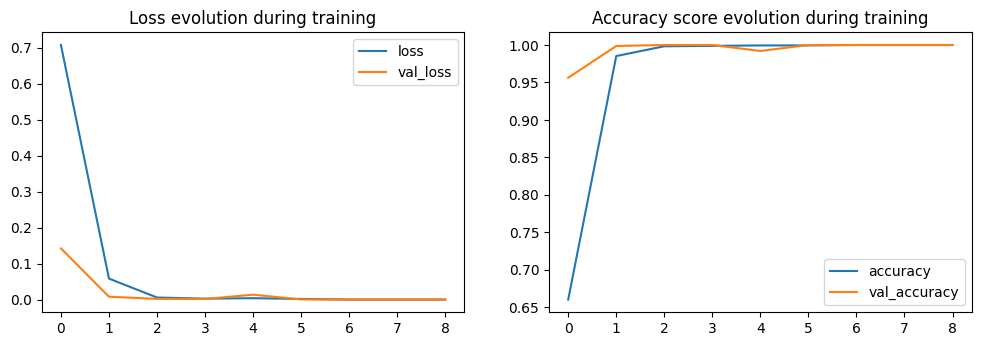
\includegraphics[scale = 0.48]{dl-figures/cnn-ex-1-learning-curves.png}
    \label{figure:cnn-ex-1-learning-curves}
\end{figure}

\lstinputlisting[firstline=169,lastline=203]{dl-scripts/cnn-ex1-colab.py}

\begin{figure}[h]
    \centering
    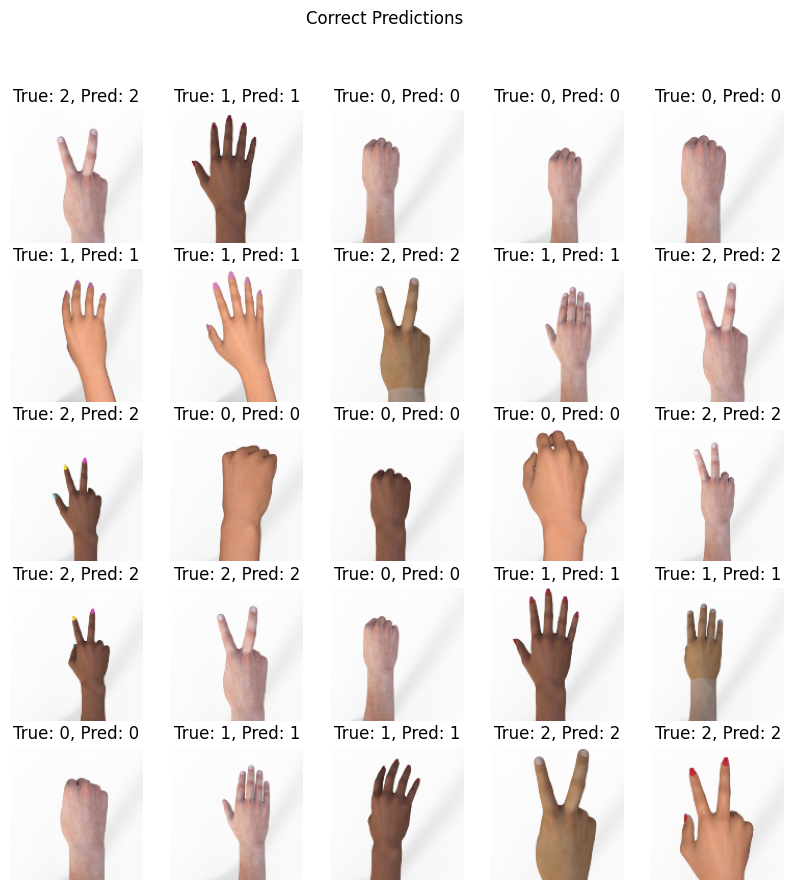
\includegraphics[scale = 0.48]{dl-figures/cnn-ex-1-correct.png}
    \label{figure:cnn-ex-1-learning-curves}
\end{figure}

\begin{figure}[h]
    \centering
    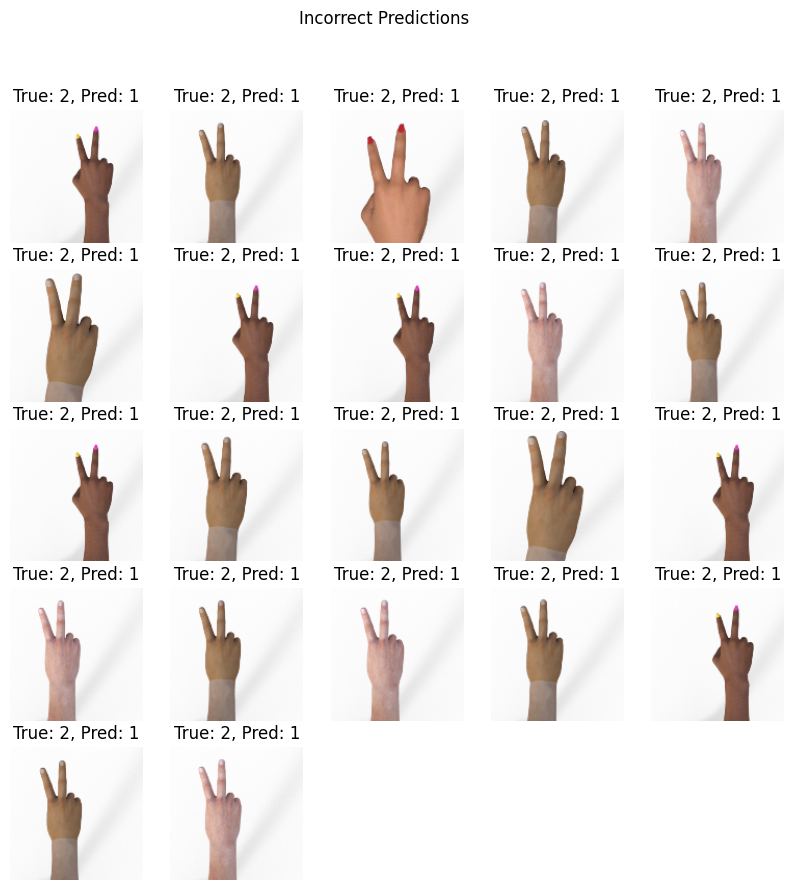
\includegraphics[scale = 0.48]{dl-figures/cnn-ex-1-incorrect.png}
    \label{figure:cnn-ex-1-learning-curves}
\end{figure}

Look at the images that were classified incorrectly. It seems that the model's most significant weakness is misclassifying scissors as paper. Do you notice anything about these scissor images compared to the scissor and paper images in the correct predictions? How could the model potentially be improved?

\section{Recurrent Neural Networks}

\section{Generative Models}

\subsection{Generative Adversarial Neural Networks}

\subsection{Variational Autoencoders}

\subsection{Quantization}

% can quantize weights or biases

% linear quantization ( see L4 quantization theory)

% example - 32-bit to 8-bit

% quanto library



\end{document}